\documentclass{beamer}

\usepackage{subcaption}
\usepackage{tikz}
\usetikzlibrary{arrows,petri,topaths}
\usepackage{tkz-berge}

\usetheme{ccc}

\newcommand{\includeressource}[2][]{\includegraphics[#1]{../resources/pdf/#2}}

\begin{document}

\title{Faster MPSoC Task Mapping via\\Symmetry Reduction}
\author{Timo Nicolai\\\texttt{timo.nicolai@mailbox.tu-dresden.de}}

\begin{frame}
\titlepage
\end{frame}

\begin{frame}
  \frametitle{Problem Statement}

  \begin{center}
    \includeressource[width=.5\linewidth]{regular_mesh_m_n.pdf}
  \end{center}
\end{frame}

\begin{frame}
  \frametitle{Problem Statement}

  \begin{center}
    \includeressource[width=.3\linewidth]{regular_mesh_m_n.pdf}
  \end{center}

  \begin{itemize}
    \item<1-> Want to intelligently map tasks to processing elements
    \item<2-> Best choice depends on underlying optimality criteria
    \item<3-> Need to perform costly simulation!
  \end{itemize}
\end{frame}

\begin{frame}
  \frametitle{Symmetry Reduction}

  \begin{itemize}
    \setlength\itemsep{.5cm}
    %
    \item<1-> One approach:
      \begin{itemize}
        \item<1-> Generate promising mappings based on previous simulations
        \item<2-> $\rightarrow$ Traverse search space ``intelligently''
      \end{itemize}
    \item<3-> Another approach:
      \begin{itemize}
        \item<3-> Partition search space into mappings equivalent \textit{by symmetry}
        \item<4-> Only work with representative of every equivalence class
        \item<5-> $\rightarrow$ ``Collapse'' search space
       \end{itemize}
  \end{itemize}
\end{frame}

\begin{frame}
  \frametitle{Symmetry Reduction}

  \begin{figure}
    \centering
    %
    \begin{subfigure}{.3\textwidth}
      \begin{overprint}
        \onslide<1>\includeressource[width=\textwidth]{%
          regular_mesh_4_4_mapping1_noarrow.pdf}
        \onslide<2>\includeressource[width=\textwidth]{%
          regular_mesh_4_4_mapping1.pdf}
      \end{overprint}
    \end{subfigure}
    %
    \hspace*{.5cm}
    %
    \begin{subfigure}{.3\textwidth}
      \includeressource[width=\textwidth]{regular_mesh_4_4_mapping2.pdf}
    \end{subfigure} \\
    %
    \vspace{.5cm}
    %
    \begin{subfigure}{.3\textwidth}
      \includeressource[width=\textwidth]{regular_mesh_4_4_mapping4.pdf}
    \end{subfigure}
    %
    \hspace*{.5cm}
    %
    \begin{subfigure}{.3\textwidth}
      \begin{overprint}
        \onslide<1>\includeressource[width=\textwidth]{%
          regular_mesh_4_4_mapping5_noarrow.pdf}
        \onslide<2>\includeressource[width=\textwidth]{%
          regular_mesh_4_4_mapping5.pdf}
      \end{overprint}
    \end{subfigure}
  \end{figure}
\end{frame}

\begin{frame}
  \frametitle{Inspirations and Contributions}

  \begin{itemize}
    \item<1-> Original idea: \cite{Goens}
    \item<2-> Theoretical foundations: \cite{Holt} and \cite{Mitchell}
    \item<3-> Important optimizations: \cite{Donaldson}
    \item<4-> Resulting framework: \cite{mpsym}
  \end{itemize}
\end{frame}

\begin{frame}
  \frametitle{Representing Symmetries I: Graph Automorphisms}

  \begin{definition}<1->
    Given two graphs $G = (V_G, E_G)$ and $H = (V_H, E_H)$, an
    \textbf{isomorphism} from $G$ to $H$ is a bijection $i: V_G \rightarrow V_H$
    with:
    $$
      \{x,y\} \in E_G \Leftrightarrow \{i(x),i(y)\} \in E_H
    $$
  \end{definition}

  \begin{definition}<2->
    An \textbf{automorphism} is an isomorphism from a graph $G$ to iself.
  \end{definition}

  \begin{definition}<3->
    A \textbf{permutation} is a bijection from a set to itself.
  \end{definition}
\end{frame}

\begin{frame}
  \frametitle{Representing Symmetries I: Automorphisms}

  \only<1>{
    \begin{figure}
      \centering
      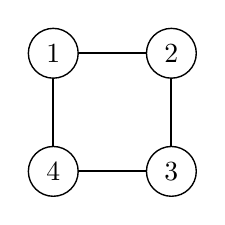
\begin{tikzpicture}
        % vertices
        \Vertex[x=0,y=0,L=$1$]{1}
        \Vertex[x=1.5,y=0,L=$2$]{2}
        \Vertex[x=1.5,y=-1.5,L=$3$]{3}
        \Vertex[x=0,y=-1.5,L=$4$]{4}
        % edges
        \Edge(1)(2)
        \Edge(2)(3)
        \Edge(3)(4)
        \Edge(4)(1)
      \end{tikzpicture}
    \end{figure}
  }

  \only<2>{
    \begin{figure}
      \centering
      \begin{subfigure}{.2\paperwidth}
        \centering
        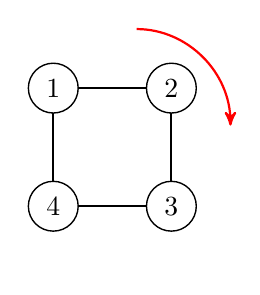
\begin{tikzpicture}[baseline=(current bounding box.center)]
          % vertices
          \Vertex[x=0,y=0,L=$1$]{1}
          \Vertex[x=1.5,y=0,L=$2$]{2}
          \Vertex[x=1.5,y=-1.5,L=$3$]{3}
          \Vertex[x=0,y=-1.5,L=$4$]{4}
          % edges
          \Edge(1)(2)
          \Edge(2)(3)
          \Edge(3)(4)
          \Edge(4)(1)
          % arrow
          \Vertex[empty,x=1,y=0.75]{x}
          \Vertex[empty,x=2.25,y=-0.5]{y}
          \tikzstyle{EdgeStyle}=[post, bend angle=45, bend left, style=thick]
          \Edge[color=red](x)(y)
          % dummy
          \Vertex[empty,x=1,y=-2.25]{x}
        \end{tikzpicture}
      \end{subfigure}
      %
      \Large$\Rightarrow$\normalsize
      %
      \begin{subfigure}{.2\paperwidth}
        \centering
        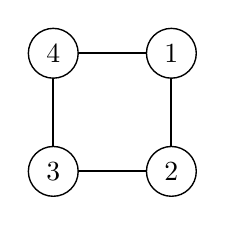
\begin{tikzpicture}[baseline=(current bounding box.center)]
          % vertices
          \Vertex[x=0,y=0,L=$4$]{1}
          \Vertex[x=1.5,y=0,L=$1$]{2}
          \Vertex[x=1.5,y=-1.5,L=$2$]{3}
          \Vertex[x=0,y=-1.5,L=$3$]{4}
          % edges
          \Edge(1)(2)
          \Edge(2)(3)
          \Edge(3)(4)
          \Edge(4)(1)
        \end{tikzpicture}
      \end{subfigure}
      %
      \Large$\Rightarrow$\makebox[.2\paperwidth]{$\ (1\ 2\ 3\ 4)$\hfill}\normalsize
      %
      \\
      %
      \begin{subfigure}{.2\paperwidth}
        \centering
        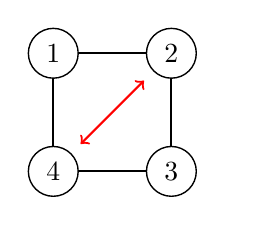
\begin{tikzpicture}[baseline=(current bounding box.center)]
          % vertices
          \Vertex[x=0,y=0,L=$1$]{1}
          \Vertex[x=1.5,y=0,L=$2$]{2}
          \Vertex[x=1.5,y=-1.5,L=$3$]{3}
          \Vertex[x=0,y=-1.5,L=$4$]{4}
          % edges
          \Edge(1)(2)
          \Edge(2)(3)
          \Edge(3)(4)
          \Edge(4)(1)
          % arrow
          \tikzstyle{EdgeStyle}=[pre and post, shorten <=5pt,shorten >=5pt, style=thick]
          \Edge[color=red](2)(4)
          % dummy
          \Vertex[empty,x=2.25,y=-0.75]{x}
        \end{tikzpicture}
      \end{subfigure}
      %
      \Large$\Rightarrow$\normalsize
      %
      \begin{subfigure}{.2\paperwidth}
        \centering
        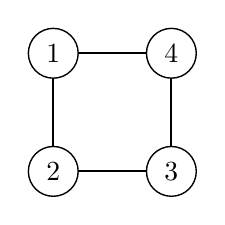
\begin{tikzpicture}[baseline=(current bounding box.center)]
          % vertices
          \Vertex[x=0,y=0,L=$1$]{1}
          \Vertex[x=1.5,y=0,L=$4$]{2}
          \Vertex[x=1.5,y=-1.5,L=$3$]{3}
          \Vertex[x=0,y=-1.5,L=$2$]{4}
          % edges
          \Edge(1)(2)
          \Edge(2)(3)
          \Edge(3)(4)
          \Edge(4)(1)
        \end{tikzpicture}
      \end{subfigure}
      %
      \Large$\Rightarrow$\makebox[.2\paperwidth]{$\ (2\ 4)$\hfill}\normalsize
    \end{figure}
  }
\end{frame}

\begin{frame}
  \frametitle{Representing Symmetries II: Automorphism Groups}

  \begin{itemize}
    \item Set of \textit{all} graph automorphisms:
      \begin{itemize}
        \item<2-> Closed under \textit{composition} and \textit{inversion}
        \item<3-> Representable by \textit{permutation group}
      \end{itemize}
  \end{itemize}

  \begin{definition}<4->
    A \textbf{group} is a tuple $(G, \circ: G \times G \rightarrow G)$ which
    satisfies:
    %
    \begin{itemize}
      \item associativity
      \item existence of (unique) identity
      \item existence of (unique) inverse
    \end{itemize}
  \end{definition}
\end{frame}

\begin{frame}
  \frametitle{Representing Symmetries III: BSGS Representation}

  \begin{itemize}
    \setlength\itemsep{.5cm}
    %
    \item<1-> Permutation group representation should allow us to:
      \begin{itemize}
        \item Iterate over all $g \in G$
        \item Test whether $g \in G$
      \end{itemize}
    \item<2-> Generating set $S$ with $G = \langle S \rangle$:
      \begin{itemize}
        \item Enumeration only via inefficient fixed-point algorithm
        \item Membership testing only via complete enumeration
      \end{itemize}
    \item<3-> \textit{Base and strong generating set (BSGS)}:
      \begin{itemize}
        \item Enumeration in $O(|G|)$
        \item Membership testing in $O(|B|)$
      \end{itemize}
  \end{itemize}
\end{frame}

\begin{frame}
  \frametitle{Representing Symmetries III: BSGS Representation}

  For a permutation group $G$:

  \vspace{.5cm}

  \begin{definition}<1->
    A \textbf{BSGS} is a tuple $(B = (\beta_1, \dots, \beta_k), S)$ which satisfies:
    %
    \begin{itemize}
      \item $B$ is not \textit{stabilized} by any $g \in G$
      \item $G = \langle S \rangle$ and $G^{(i)} = \langle S^{(i)} \rangle =
            \langle S \cap G^{(i)} \rangle$
    \end{itemize}
  \end{definition}

  \vspace{.5cm}

  \visible<2>{
    $G^{(i)}$ are the \textit{basic stabilizers} with:
    $$
      1 = G^{(k+1)} \leq G^{(k)} \leq \dots \leq G^{(1)} = G
    $$
  }
\end{frame}

\begin{frame}
  \frametitle{References}

  \bibliography{bibliography}
  \bibliographystyle{apalike}
\end{frame}

\end{document}
